\documentclass[../piano-di-progetto.tex]{subfiles}

\begin{document}

  \subsection{III incremento}

  \subsubsection{Prospetto orario}
 Durante il terzo incremento, la distribuzione oraria è la seguente:
  \begin{table}[H]
    \centering
    \begin{tabular}{lccccccc}
    \rowcolor{lightgray}
    \textbf{Nominativo}       & \textbf{Re} & \textbf{Am} & \textbf{An} & \textbf{Pt} & \textbf{Pr} & \textbf{Ve} & \textbf{Ore totali} \\
Sofia Bononi              & -           & -           & -           & -           & 4           & 1           & 5                   \\
Enrico Buratto            & -           & -           & -           & 4           & -           & -           & 4                   \\
Ian Nicolas Di Menna      & -           & -           & 1           & -           & 4           & -           & 5                   \\
Alessandro Franchin       & -           & 2           & -           & -           & -           & 1           & 3                   \\
Enrico Galdeman           & 2           & -           & -           & -           & -           & 2           & 4                   \\
Nicholas Miazzo           & -           & -           & -           & -           & -           & 4           & 4                   \\
Marco Nardelotto          & -           & -           & 2           & -           & -           & 2           & 4                   \\
\textbf{Ore totali ruolo} & \textbf{2}  & \textbf{2}  & \textbf{3}  & \textbf{4}  & \textbf{8}  & \textbf{10} & \textbf{29}        
    
    \end{tabular}
    \caption{Distribuzione oraria del terzo incremento}
  \end{table}


  Per facilitare la lettura della distribuzione oraria, i dati vengono rappresentati graficamente mediante il seguente istogramma:
  \begin{figure}[H]
    \centering
    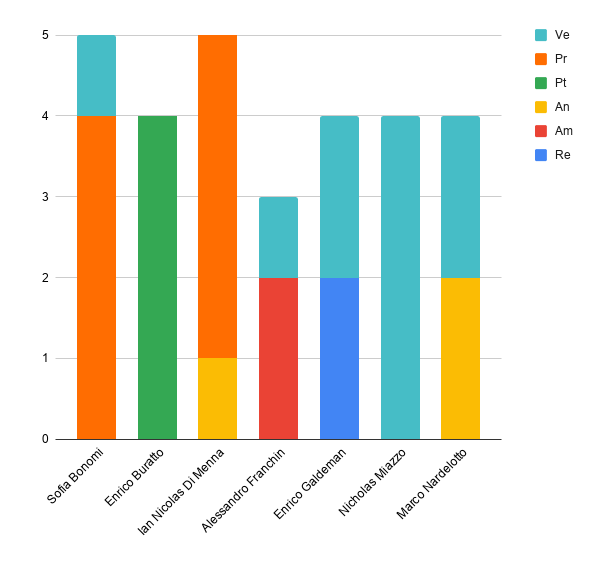
\includegraphics[width=12cm]{img/ore-3-incr.png}
    \caption{Istogramma della distribuzione oraria del terzo incremento}
    \label{fig:ore-componente-progettazione}
  \end{figure}

  \subsubsection{Prospetto economico}
  In questo periodo, la suddivisione oraria e i costi per ruolo è la seguente:

  \begin{table}[H]
    \centering
    \begin{tabular}{lcc}
      \rowcolor{lightgray}
      \textbf{Ruolo}  & \textbf{Ore previste} & \textbf{Costo}    \\
Responsabile    & 2                     & € 60,00           \\
Amministratore  & 2                     & € 40,00           \\
Analista        & 3                     & € 75,00           \\
Progettista     & 4                     & € 88,00           \\
Programmatore   & 8                     & € 120,00          \\
Verificatore    & 10                    & € 150,00          \\
\textbf{Totale} & \textbf{29}           & \textbf{€ 533,00}
    \end{tabular}
    \caption{Prospetto economico del terzo incremento}
  \end{table}


  Per facilitare la lettura della suddivisione oraria per ruolo, i dati vengono rappresentati graficamente mediante il seguente areogramma:
  \begin{figure}[H]
    \centering
    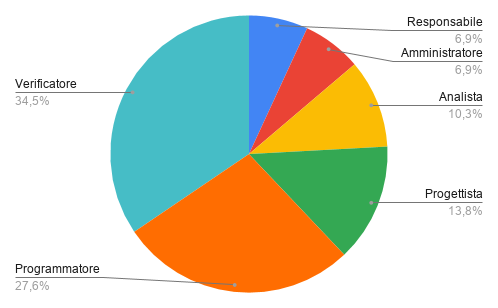
\includegraphics[width=12cm]{img/ruoli-3-incr.png}
    \caption{Areogramma della suddivisione dei ruoli del terzo incremento}
    \label{fig:ore-ruolo-progettazione}
  \end{figure}



\end{document}
